%% supplement.tex -- supplementary material for the IEEE T-BIOM submission.
%% Standalone; compile: pdflatex, bibtex, pdflatex twice.
\documentclass[journal]{IEEEtran}

\usepackage[T1]{fontenc}
\usepackage[utf8]{inputenc}
\usepackage{cite}
\usepackage{array}
\usepackage{booktabs}
\usepackage{enumitem}
\usepackage{xcolor}
\usepackage{amsmath,amssymb}
\usepackage{graphicx}
\graphicspath{{../../../shared/figures/}}
\usepackage[hidelinks]{hyperref}

\newcommand{\dgr}{$\leftrightarrow$}
\newcommand{\mainsec}[1]{main Sec.~#1}
\newcommand{\maintab}[1]{main Table~#1}

\begin{document}

\title{Supplementary Material:\\ Cross-Age Face Verification from Mined Same-Person Social-Media Pairs}
\author{Danil~F.~Volkhin and Ivan~S.~Kopylov}
\markboth{IEEE Transactions on Biometrics, Behavior, and Identity Science --- Supplementary Material}{}
\maketitle

\noindent This supplement collects material that supports, but need not occupy, the main paper:
(S\ref{sec:claims}) an explicit claims-vs-evidence map; (S\ref{sec:audit}) a consolidated audit of
the automatic (LLM / clustering / dedup) supervision components and the protocol required for a
planned prespecified multi-annotator audit; (S\ref{sec:quality}) the data-quality funnel and
distributions; (S\ref{sec:card}) a model/data card; (S\ref{sec:published}) the non-comparable
published-results map; and (S\ref{sec:figs}) secondary tables and figures. References prefixed
``main'' point to the main paper; all other section, table and figure references are local.

\section{Historical Protocol Comparisons}\label{sec:legacy-main}
These are secondary historical comparisons, not the corrected FG-NET primary endpoint.
The reported LFW accuracies use legacy interleaved splits rather than official contiguous
View-2 folds; the separate new source-bound evaluation is in Table~\ref{tab:lfw-bound}.
The legacy aligned cache also lacks
verified person/row provenance, so its existing intervals must not be called subject-level.
\begin{table*}[!t]
\renewcommand{\arraystretch}{1.2}
\caption{Historical random-impostor comparisons: weak FaceNet frozen vs.\ $+$pairs, three seeds, curated data. These FG-NET rows are not the corrected primary endpoint (main paper's corrected endpoint table). Pre-clean gain is shown for reference.}
\label{tab:legacy-main}
\centering
\footnotesize
\begin{tabular}{@{}lcccc@{}}
\toprule
Metric & Frozen & $+$pairs (mean $\pm$ std) & Gain & (Pre-clean gain) \\
\midrule
FG-NET large-gap & 0.7361 & 0.8484 $\pm$ 0.0007 & \textbf{$+$0.1124} & $+$0.1215 \\
FG-NET ROC & 0.8955 & 0.9230 $\pm$ 0.0006 & $+$0.0275 & $+$0.0277 \\
our.25+ (internal) & 0.6403 & 0.8348 $\pm$ 0.0027 & \textbf{$+$0.1946} & $+$0.1677 \\
our.overall (internal) & 0.8363 & 0.9163 $\pm$ 0.0009 & $+$0.0801 & $+$0.0764 \\
LFW accuracy & 0.9640 & 0.9679 $\pm$ 0.0002 & $+$0.0039 & n/a \\
AgeDB-30 ROC & 0.9530 & 0.9462 $\pm$ 0.0013 & $-$0.0068 & $-$0.0155 \\
CALFW ROC & 0.9482 & 0.9489 $\pm$ 0.0014 & $+$0.0007 & $-$0.0030 \\
CACD-VS ROC & 0.9948 & 0.9947 $\pm$ 0.0002 & $-$0.0001 & n/a \\
\bottomrule
\end{tabular}
\end{table*}

\section{Claims vs.\ Evidence}\label{sec:claims}
Table~\ref{tab:claims} maps every substantive claim to its evidence and its scope, separating what
is \emph{established within the attribution protocol} from what is \emph{not established}. The intent
is to make the bounded reading explicit and to forestall over-generalization.

\begin{table*}[!t]
\renewcommand{\arraystretch}{1.15}
\caption{Claims vs.\ Evidence. ``Est.'' = established within the weak/medium-backbone attribution
protocol of the main paper; ``Bounded'' = holds only under stated conditions; ``Open'' = not
established / out of scope.}
\label{tab:claims}
\centering
\footnotesize
\begin{tabular}{@{}p{0.38\textwidth}p{0.40\textwidth}p{0.16\textwidth}@{}}
\toprule
Claim & Evidence (main paper) & Status \\
\midrule
Mined ``then/now'' pairs improve large-gap ($\geq$25\,y) cross-age verification under endpoint-age matching &
FG-NET 25+ ROC-AUC $0.8023\!\to\!0.8491{\pm}0.0017$; mean checkpoint gain CI $[+0.0074,+0.0916]$ conditional on fixed weights (Table~\ref{tab:fgnet-roc-v2}); benchmark-overlap adjudication remains pending & Bounded \\
The gain is \emph{targeted}, not a uniform verification gain &
Historical AgeDB-30 AUC decreases; source-bound CACD-VS loses accuracy/TAR@FAR1\% and raises EER (S\ref{sec:cacd-serial}). Source-bound LFW supports AUC gain, but accuracy/low-FAR gain CIs include zero (S\ref{sec:lfw-bound}) & Bounded \\
Explicit caption age anchors add little within the tested same-post ablation &
Pre-clean ablation: age anchors add $+0.009$ on the original 25+ bucket (\mainsec{V-A}); this does not isolate the causal source effect & Bounded \\
The full-image-budget within-VK control does not establish long-gap superiority &
Replacement three-checkpoint CROSS--LOW 25+ AUC $+0.0031$, paired subject CI $[-0.0198,+0.0261]$ (Table~\ref{tab:oriented-source}); historical $+0.0257$ had unequal image budgets. Completed fixed-permutation noise sensitivity does not replace generic/co-occurrence controls or identity adjudication & Bounded \\
Real mined pairs outperform the tested FRAN controls under the historical protocol &
$+$real $0.848$ vs.\ FRAN $0.727$ and gap-matched FRAN-gm $0.759$ ($+0.089$); native-resolution control (\mainsec{V-B}) & Est. \\
Tested objectives have similar historical point estimates &
ArcFace $0.851$, contrastive $0.848$ and sub-center ArcFace $0.851$ on the original protocol; no objective-equivalence test (\mainsec{V-F}) & Bounded \\
The tested noise-robust objective has no observed point-estimate advantage &
Sub-center and vanilla ArcFace both report $0.851$ on historical FG-NET large-gap; this is not an equivalence or label-noise guarantee (\mainsec{V-F}) & Bounded \\
Endpoint-age-matched negatives preserve a bounded weak-backbone AUC gain, not a uniform operating-point gain &
Internal 154/154 pairs: ROC-AUC $0.768\!\to\!0.833$ ($\Delta=+0.065$, paired recorded-person CI $[+0.005,+0.131]$). ROC-v2 TAR: 1\% $0.338\!\to\!0.403$; 0.1\% $0.325\!\to\!0.253$; both change CIs include zero (Table~\ref{tab:internal-roc-v2}) & Bounded; identity audit pending. \\
An earlier scaling sweep suggested data efficiency &
${\approx}96\%$ of the recorded gain at 10\% of identities, but intermediate checkpoints were overwritten and a schema-v2 rerun is pending (\mainsec{V-D}) & Exploratory. \\
Apparent-demographic gains are observed under the historical internal protocol &
Stratified internal AUC (all gain CIs $>0$) and the historical threshold audit (\mainsec{V-G}); this does not establish improvement in every external error stratum & Bounded \\
About half of the raw ``positives'' were near-duplicates &
$65{,}897\!\to\!31{,}865$ ($-52\%$), stable over cosine $0.93$--$0.97$ (\mainsec{III-D}, \maintab{V}) & Est. \\
The gain transfers beyond the originating platform, in \emph{both} directions &
VK$\to$Reddit overall ROC-AUC $0.718\!\to\!0.757{\pm}0.008$; Reddit$\to$VK FG-NET large-gap $0.736\!\to\!0.779{\pm}0.004$ (three seeds; 220-person source); small, noisy sets (\mainsec{V-I}) & Bounded \\
The contribution is specific to weak/medium backbones &
An exploratory one-seed curve shows null/negative strong-backbone gains; the planned fixed-budget mechanism matrix is incomplete (\mainsec{V-C}) & Open (experiment pending) \\
Platform-agnostic / cross-cultural generalization & one platform family, then/now format; single non-VK test & Open \\
Drop-in upgrade to a general-purpose verifier & mixed AUC/accuracy/low-FAR trade-offs; large-gap primary endpoint uses small FG-NET & Open (excluded) \\
Human-grade label-noise guarantee & corpus-scale automatic cross-checks only; prespecified multi-annotator audit not yet completed (S\ref{sec:audit}) & Open \\
Restricted-stage comparison, not full-method parity & three-seed MTLFace/CACon-CP variants; joint synthesis and final-linear stages remain incomplete & Bounded \\
Legal/ethical clearance for biometric processing & formal institutional determination not yet obtained (\mainsec{VIII}) & Open (institutional gate) \\
\bottomrule
\end{tabular}
\end{table*}

\section{Consolidated Audit of the Automatic Supervision}\label{sec:audit}
The supervision is \emph{naturally} (not human-) supervised, so its automatic components are potential
hidden label noise. Table~\ref{tab:auditfull} consolidates the corpus-scale automatic cross-checks
reported across the main paper. None of these rows is accuracy against human ground truth. Before
resubmission, the pipeline requires the prepared audit by two independent annotators on held-out
samples of age extraction, group integrity, positive pairs, cluster merges and near-duplicate removals.
The frozen pack contains 400 items per target, independent random orders, opaque copied-image names,
a separately held source/automatic-decision key and an adjudication template; it was generated only
after thresholds were fixed. For age extraction, the pack
reconstructs the original post and photo order (rather than inheriting a caption after cross-post person
merging), identifies a zero-based target image, and forbids appearance-based age estimation.
The aggregate validator artifact \texttt{metrics/human\_audit\_pack\_validation.json} confirms
2,000 tasks per annotator, five 400-item strata, 5,112 checksum-valid opaque image copies and zero
source-identifier, automatic-decision or cross-stratum source-image leaks. Group integrity is balanced
between 200 automatically accepted and 200 automatically rejected pre-prune groups. The dedup stratum
contains 272 automatic near-duplicate and 128 automatic distinct-photo decisions spanning cosine
0.963--0.976 around the 0.97 production threshold; all 5,112 source images are disjoint. Downstream intervals use source-component cluster
resampling (equivalent to item resampling for this fully disjoint pack). The validator
artifact contains no images or row-level task content.

\begin{table*}[!t]
\renewcommand{\arraystretch}{1.25}
\caption{Consolidated corpus-scale checks of the automatic supervision. ``Reference'' identifies the
automatic comparator or proxy; none of these measurements uses human ground truth. $n$ is the checked
population. A prespecified multi-annotator audit remains required before resubmission.}
\label{tab:auditfull}
\centering
\footnotesize
\begin{tabular}{@{}p{0.26\textwidth}rp{0.20\textwidth}p{0.30\textwidth}@{}}
\toprule
Audit target & $n$ & Reference & Result \\
\midrule
Age extraction (LLM vs.\ regex) & 33{,}697 captions & automatic cross-check & $78.1\%$ exact/both-empty agreement; $15.5\%$ different non-empty ages, $3.4\%$ LLM-only, $3.0\%$ regex-only; \maintab{III} \\
Group integrity (LLM classifier) & 33{,}697 posts & automatic (LLM) & $92.8\%$ single-person, $6.0\%$ multi-person, $1.0\%$ unknown, $0.2\%$ meme; \maintab{IV} \\
Apparent-gender consistency diagnostic & multi-face groups & automatic proxy & $2{,}919$ pre-prune groups below $0.6$; $2{,}866$ retained; not a pruning rule \\
Near-duplicate inflation (within-person dedup) & $65{,}897$ raw positives & automatic (embedding) & $-52\%$ ($\to 31{,}865$); stable for cosine $0.93$--$0.97$; \maintab{V} \\
Recorded-person merging & 27{,}487 mapped groups & automatic (embedding) & $21{,}847$ components at cosine $0.85$; one additional singleton fallback gives $21{,}848$ pre-prune groups \\
Independent embedding sensitivity & 27{,}487 post-groups & FaceNet/CASIA sweep & $21{,}484$ persons at cosine $0.85$ (1.7\% below ArcFace); dedup reduction 52.1--53.4\% at cosine $0.90$--$0.97$ \\
\bottomrule
\end{tabular}
\end{table*}

The rows have versioned aggregate evidence, not a verified end-to-end replay of historical curation.
They establish internal consistency only, not human-validated label precision. The held-out pack and scorer
are complete, but both independent response files and adjudication remain external human work. Before
annotation, predictions were frozen for the GigaChat pipeline, deterministic regex and a fully local
character-ngram ridge baseline trained on 32{,}279 non-audit automatic anchors (all audit rows excluded;
regex coverage on the audit pack is 59.0\%). These weak targets make the local model a reproducibility
comparator, not ground truth. The scorer reports system-specific coverage, exact match, within-one-year
accuracy and age MAE; Cohen's $\kappa$; precision/recall/F1 when both automatic decisions are sampled;
and PPV for accept-only positive/merge strata, all with bootstrap 95\% confidence intervals. No quantitative
human-validation claim is made until both response files and adjudication are frozen.

The machine-readable artifact index, \texttt{metrics/publication\_artifact\_index.json}, enumerates
experiment manifests, their commands, parameters, git state and output checksums. It fails closed by
listing missing expected manifests, checksum mismatches and incomplete semantic campaign gates; the working index is therefore not marked
complete while the strong-backbone and remaining legacy-table reruns are still open.
A separate \texttt{publication-evidence.zip} contains eight selected aggregate results,
sanitized manifest projections and a checksum certificate distinguishing original from
exported bytes. Direct original inputs and outputs are verified locally; private records
are represented by counts, not redistributed. This is partial aggregate evidence, not
full experiment reproducibility or clearance of the outstanding publication gates.
A separate \texttt{curation-evidence.zip} provides three aggregate audits (record lineage,
global-ID reconstruction and constituent-caption sensitivity), three count-only sanitized
manifests and a checksum certificate. It excludes the private candidate list and original
record paths/digests. Reconstruction is not recovered historical provenance; cached automatic
labels are not human gold. Disclosure review and adjudication remain pending.

\paragraph{Strong-backbone matrix protocol.}
The confirmatory AdaFace IR-101/WebFace12M study crosses learning rate
$\{10^{-6},10^{-5}\}$, trainable scope $\{\text{head},\text{tail},\text{full}\}$ and
$\{\text{random},\text{look-alike}\}$ negatives over seeds 42/1/2. Head denotes the final
BN--FC--BN output layer; tail additionally unfreezes the last residual body block; full unfreezes the
entire backbone. The ongoing fixed-budget campaign requests eight epochs and selects the last
epoch, without validation-based early stopping. BatchNorm running statistics are frozen in every
scope; affine parameters follow the declared trainable scope. Requested, executed and selected epochs
are recorded separately. Earlier best-validation checkpoints with adaptive BatchNorm are exploratory,
not cells of this confirmatory matrix. Both negative arms use the same held-out evaluation pairs.
Completed fixed-last head/tail cells record training loss, validation AUC and mean gradient norm;
validation loss was not collected and cannot be recovered from AUC. Partial native-bound diagnostics
measure linear CKA, cosine drift, descriptive cosine separation and per-image age regression using
person-disjoint folds, fit-only scaling and matched-denominator mean/median constant controls.
Subject intervals condition on fixed checkpoints and probe predictions, not training-seed populations.
These measurements do not establish age removal or a mechanism; an age-gap probe is not age decoding.
Corrected endpoint-age-matched FG-NET evaluation is partial, not a completed matrix. The interpretation
is fixed before reading the complete matrix: a random-impostor ceiling requires near-perfect frozen
random AUC but does not imply task-level ceiling when look-alike AUC is low; insufficient plasticity is
supported only if widening scope or increasing LR increases representation change and restores transfer;
catastrophic forgetting requires broad external degradation rather than a task-specific large-gap drop.
Completed cells will provide machine-readable per-seed trajectories and deltas; the full matrix
is not yet available, and a negative fine-tuning result will be retained.

\section{Partial Common-Image Feature Diagnostics}\label{sec:common-image-feature-diagnostics}
Tables~\ref{tab:common-mechanism-strong} and~\ref{tab:common-mechanism-weak}
describe nine AdaFace checkpoints: the initial six random/head--tail/LR $10^{-6}$
and random/head/LR $10^{-5}$ seeds 42/1/2, plus
the three cached FaceNet checkpoints on the same 650 images and 5{,}308
endpoint-age-matched pairs from 82 recorded people. Exact pair arrays and
image metadata agree across bindings; this is not human identity clearance.
Each family is compared with its own frozen reference. Different architectures,
preprocessing and unverified weak training history preclude a controlled causal
comparison between families. Repeated weak bindings are rendered once.

Head changes are smaller than tail changes in these descriptive CKA/drift
measurements, but neither quantity is a measure of improved verification.
All nine strong separation-change intervals are below zero; the three weak
intervals are above zero. Tail age-MAE-change intervals are below zero,
as are the LR $10^{-5}$ head seed1/2 intervals; the remaining head and weak
age-MAE-change intervals include zero. Lower age MAE
means easier age decoding, not age removal. These nominal paired subject
intervals condition on fixed checkpoints and fixed out-of-fold predictions;
probes are not refitted within resamples and no multiplicity correction is
applied. They are not intervals of seed means or training-seed populations.

Table~\ref{tab:age-probe-absolute-points} separates image-weighted and
equal-person MAE and includes fit-only mean/median constant references.
It covers the same nine strong checkpoints as the feature tables.
Its fourteen unique model points are deduplicated from repeated native records,
not independent replications. The strong frozen linear probe has a larger
point error than the constants at these fixed settings; this does not prove
absence of age information. No new absolute-error interval or significance
test is supplied. These diagnostics do not identify saturation, inadequate
plasticity or catastrophic forgetting; validation loss, the full matrix and
broader external checks remain open.

% BEGIN GENERATED COMMON FEATURE V2
\begin{table*}[!t]
\caption{Strong arm: 9 of 36 expected tuned checkpoints, each conditional on its own fixed checkpoint (descriptive, not the full matrix). Frozen reference separation SMD is 3.3424 (95\% CI $[3.1406,3.5781]$), the same bound reference in every row. $\Delta$MAE and SMD deltas are tuned minus frozen; each interval is the paired subject/endpoint bootstrap interval for this checkpoint, not a seed mean and not an ensemble. Age intervals hold OOF probe predictions fixed, with no probe refitting. Lower age MAE means easier age decoding, not age removal. Descriptive only: no mechanism decision, no training-seed population inference, no identity-independence clearance and no multiplicity correction; not deployment-calibrated.}
\label{tab:common-mechanism-strong}
\centering\scriptsize
\resizebox{\textwidth}{!}{%
\begin{tabular}{@{}lrrrrrrr@{}}
\toprule
Checkpoint & CKA & Cos.\ drift & Age $\Delta$MAE & Age $\Delta$MAE 95\% CI & Sep.\ SMD & Sep.\ $\Delta$SMD & Sep.\ $\Delta$95\% CI \\
\midrule
random, head, LR $10^{-5}$, seed 1 & 0.6715 & 0.3757 & -1.2625 & $[-2.4808,-0.2478]$ & 2.6011 & -0.7413 & $[-0.9322,-0.5181]$ \\
random, head, LR $10^{-5}$, seed 2 & 0.6734 & 0.3758 & -1.3266 & $[-2.5444,-0.3325]$ & 2.5983 & -0.7441 & $[-0.9376,-0.5182]$ \\
random, head, LR $10^{-5}$, seed 42 & 0.6734 & 0.3759 & -0.9989 & $[-2.2444,+0.0367]$ & 2.6113 & -0.7311 & $[-0.9243,-0.5048]$ \\
random, head, LR $10^{-6}$, seed 1 & 0.9470 & 0.0570 & -0.1671 & $[-0.6659,+0.3229]$ & 3.2063 & -0.1362 & $[-0.2470,-0.0142]$ \\
random, head, LR $10^{-6}$, seed 2 & 0.9468 & 0.0574 & -0.1635 & $[-0.6650,+0.3315]$ & 3.2038 & -0.1386 & $[-0.2503,-0.0156]$ \\
random, head, LR $10^{-6}$, seed 42 & 0.9470 & 0.0570 & -0.1371 & $[-0.6410,+0.3588]$ & 3.2072 & -0.1352 & $[-0.2456,-0.0121]$ \\
random, tail, LR $10^{-6}$, seed 1 & 0.6002 & 0.4563 & -1.7002 & $[-2.7847,-0.5906]$ & 3.0691 & -0.2733 & $[-0.4699,-0.0590]$ \\
random, tail, LR $10^{-6}$, seed 2 & 0.6030 & 0.4543 & -1.6439 & $[-2.7657,-0.5049]$ & 3.0826 & -0.2599 & $[-0.4584,-0.0446]$ \\
random, tail, LR $10^{-6}$, seed 42 & 0.6020 & 0.4546 & -1.6610 & $[-2.7840,-0.5394]$ & 3.0797 & -0.2627 & $[-0.4562,-0.0522]$ \\
\bottomrule
\end{tabular}%
}
\end{table*}

\begin{table*}[!t]
\caption{Weak arm: the same bound weak tuned family appears in every binding and is rendered once (deduplicated, not averaged or ensembled). Frozen reference separation SMD is 1.7918 (95\% CI $[1.6217,1.9877]$). $\Delta$MAE and SMD deltas are tuned minus frozen; intervals are conditional paired subject bootstrap intervals, not a seed mean and not an ensemble. Lower age MAE means easier age decoding, not age removal. Descriptive only: no mechanism decision, no training-seed population inference and no identity-independence clearance; weak training history unverified. Age intervals hold OOF predictions fixed, without probe refitting or multiplicity correction. Different architecture/preprocessing, not a causal family comparison.}
\label{tab:common-mechanism-weak}
\centering\scriptsize
\resizebox{\textwidth}{!}{%
\begin{tabular}{@{}lrrrrrrr@{}}
\toprule
Checkpoint & CKA & Cos.\ drift & Age $\Delta$MAE & Age $\Delta$MAE 95\% CI & Sep.\ SMD & Sep.\ $\Delta$SMD & Sep.\ $\Delta$95\% CI \\
\midrule
tuned, seed 42 & 0.8896 & 0.1750 & +0.0873 & $[-0.1872,+0.3449]$ & 2.0631 & +0.2713 & $[+0.1100,+0.4236]$ \\
tuned, seed 1 & 0.8909 & 0.1670 & +0.1605 & $[-0.1255,+0.4245]$ & 2.0686 & +0.2768 & $[+0.1181,+0.4291]$ \\
tuned, seed 2 & 0.8926 & 0.1589 & +0.1719 & $[-0.1025,+0.4370]$ & 2.0767 & +0.2849 & $[+0.1309,+0.4288]$ \\
\bottomrule
\end{tabular}%
}
\end{table*}
% END GENERATED COMMON FEATURE V2

% BEGIN GENERATED ABSOLUTE AGE POINTS V3
\begin{table}[!t]
\caption{Absolute age-probe and fit-only constant MAE points (years). Strong rows cover exactly the 9 explicitly declared cells of the 36-cell (random|lookalike) x (head|tail|full) x LR $10^{-6}$/$10^{-5}$ x seed {42,1,2} matrix; every remaining cell is not rendered. The matrix stays incomplete. Weak rows use different architecture/preprocessing and unverified training history, not a controlled causal family comparison. Repeated physical probe records are deduplicated, not independent replications. Image-weighted and equal-person MAE are separate denominators; no new interval or significance test, age-removal claim, mechanism or identity-independence clearance.}
\label{tab:age-probe-absolute-points}
\centering\scriptsize
\begin{tabular}{@{}lrr@{}}
\toprule
Model/reference & Image-weighted MAE & Equal-person MAE \\
\midrule
Fit-only mean & 9.4523 & 9.3086 \\
Fit-only median & 9.1354 & 9.0775 \\
Strong frozen & 9.9156 & 10.2270 \\
Strong random head, LR $10^{-5}$, seed 1 & 8.9230 & 8.9645 \\
Strong random head, LR $10^{-5}$, seed 2 & 8.8890 & 8.9003 \\
Strong random head, LR $10^{-5}$, seed 42 & 9.1964 & 9.2281 \\
Strong random head, LR $10^{-6}$, seed 1 & 9.9099 & 10.0599 \\
Strong random head, LR $10^{-6}$, seed 2 & 9.9149 & 10.0634 \\
Strong random head, LR $10^{-6}$, seed 42 & 9.9424 & 10.0899 \\
Strong random tail, LR $10^{-6}$, seed 1 & 8.2777 & 8.5267 \\
Strong random tail, LR $10^{-6}$, seed 2 & 8.3478 & 8.5830 \\
Strong random tail, LR $10^{-6}$, seed 42 & 8.3245 & 8.5659 \\
Weak frozen & 5.7657 & 5.9908 \\
Weak, seed 1 & 5.9866 & 6.1513 \\
Weak, seed 2 & 5.9962 & 6.1627 \\
Weak, seed 42 & 5.9123 & 6.0781 \\
\bottomrule
\end{tabular}
\end{table}
% END GENERATED ABSOLUTE AGE POINTS V3

\section{Partial Fixed8 AdaFace ROC-v2}\label{sec:strong-fixed8-roc-v2}
Nine completed cells cover random negatives: head/tail at learning rate $10^{-6}$
and head at $10^{-5}$, each with seeds 42/1/2; they are not the full matrix. Overall evaluation
uses 5{,}308 pairs/82 subjects, the 25+ stratum 430 pairs/75 subjects, from the same 650 images.
Tables~\ref{tab:strong-fixed8-overall} and~\ref{tab:strong-fixed8-large-gap-25plus}
report each checkpoint separately. In the initial six LR $10^{-6}$ cells,
overall head AUC decreases; tail AUC-change intervals include zero. Overall EER
and both low-FAR TAR changes are unfavorable with nominal conditional intervals
excluding zero; all 25+ change intervals include zero for those six cells.
For all three LR $10^{-5}$ head checkpoints, 25+ AUC decreases and EER increases
with conditional intervals excluding zero; TAR at FAR 0.1\% also decreases.
The 25+ TAR-change interval at FAR 1\% includes zero for seed2, but excludes it
for seeds42/1. These are checkpoint-conditional results, not intervals of seed means.
No equivalence or mechanism follows from an
inconclusive interval. These strata share FG-NET, and identity independence remains
unverified. Source-bound generated tables do not recover missing validation loss.

% BEGIN GENERATED STRONG FIXED8 ROC V1
\begin{table*}[!t]
\caption{Overall: 9 evaluated fixed8 AdaFace checkpoints from the 36-cell matrix. Entries and paired subject intervals are per checkpoint, not a seed mean or an ensemble. No training-seed population inference, mechanism claim or identity-independence clearance. Empirical thresholds are reselected, not deployment-calibrated; no multiplicity correction.}
\label{tab:strong-fixed8-overall}
\centering\scriptsize
\begin{tabular}{@{}llrrrr@{}}
\toprule
Cell & Metric & Frozen & Tuned & Delta & Paired delta 95\% CI \\
\midrule
random/head/1e-05/s1 & ROC-AUC & 0.9896 & 0.9606 & -0.0290 & $[-0.0397,-0.0190]$ \\
random/head/1e-05/s1 & Interpolated EER & 0.0452 & 0.1010 & +0.0558 & $[+0.0364,+0.0716]$ \\
random/head/1e-05/s1 & Discrete minimax EER & 0.0452 & 0.1010 & +0.0558 & $[+0.0364,+0.0716]$ \\
random/head/1e-05/s1 & TAR@FAR=1\% & 0.8971 & 0.6654 & -0.2317 & $[-0.2788,-0.1574]$ \\
random/head/1e-05/s1 & TAR@FAR=0.1\% & 0.7931 & 0.5607 & -0.2325 & $[-0.3432,-0.1359]$ \\
random/head/1e-05/s2 & ROC-AUC & 0.9896 & 0.9604 & -0.0292 & $[-0.0397,-0.0190]$ \\
random/head/1e-05/s2 & Interpolated EER & 0.0452 & 0.0995 & +0.0543 & $[+0.0363,+0.0725]$ \\
random/head/1e-05/s2 & Discrete minimax EER & 0.0452 & 0.0995 & +0.0543 & $[+0.0363,+0.0725]$ \\
random/head/1e-05/s2 & TAR@FAR=1\% & 0.8971 & 0.6669 & -0.2302 & $[-0.2812,-0.1600]$ \\
random/head/1e-05/s2 & TAR@FAR=0.1\% & 0.7931 & 0.5452 & -0.2479 & $[-0.3635,-0.1381]$ \\
random/head/1e-05/s42 & ROC-AUC & 0.9896 & 0.9612 & -0.0284 & $[-0.0391,-0.0185]$ \\
random/head/1e-05/s42 & Interpolated EER & 0.0452 & 0.0998 & +0.0546 & $[+0.0356,+0.0709]$ \\
random/head/1e-05/s42 & Discrete minimax EER & 0.0452 & 0.0998 & +0.0546 & $[+0.0356,+0.0709]$ \\
random/head/1e-05/s42 & TAR@FAR=1\% & 0.8971 & 0.6639 & -0.2332 & $[-0.2809,-0.1591]$ \\
random/head/1e-05/s42 & TAR@FAR=0.1\% & 0.7931 & 0.5659 & -0.2272 & $[-0.3477,-0.1418]$ \\
random/head/1e-06/s1 & ROC-AUC & 0.9896 & 0.9824 & -0.0071 & $[-0.0113,-0.0031]$ \\
random/head/1e-06/s1 & Interpolated EER & 0.0452 & 0.0659 & +0.0207 & $[+0.0098,+0.0318]$ \\
random/head/1e-06/s1 & Discrete minimax EER & 0.0452 & 0.0659 & +0.0207 & $[+0.0098,+0.0318]$ \\
random/head/1e-06/s1 & TAR@FAR=1\% & 0.8971 & 0.8399 & -0.0573 & $[-0.1091,-0.0179]$ \\
random/head/1e-06/s1 & TAR@FAR=0.1\% & 0.7931 & 0.7442 & -0.0490 & $[-0.1337,-0.0045]$ \\
random/head/1e-06/s2 & ROC-AUC & 0.9896 & 0.9823 & -0.0072 & $[-0.0114,-0.0032]$ \\
random/head/1e-06/s2 & Interpolated EER & 0.0452 & 0.0663 & +0.0211 & $[+0.0099,+0.0321]$ \\
random/head/1e-06/s2 & Discrete minimax EER & 0.0452 & 0.0663 & +0.0211 & $[+0.0099,+0.0321]$ \\
random/head/1e-06/s2 & TAR@FAR=1\% & 0.8971 & 0.8399 & -0.0573 & $[-0.1091,-0.0177]$ \\
random/head/1e-06/s2 & TAR@FAR=0.1\% & 0.7931 & 0.7408 & -0.0524 & $[-0.1354,-0.0053]$ \\
random/head/1e-06/s42 & ROC-AUC & 0.9896 & 0.9825 & -0.0071 & $[-0.0113,-0.0031]$ \\
random/head/1e-06/s42 & Interpolated EER & 0.0452 & 0.0663 & +0.0211 & $[+0.0097,+0.0316]$ \\
random/head/1e-06/s42 & Discrete minimax EER & 0.0452 & 0.0663 & +0.0211 & $[+0.0097,+0.0316]$ \\
random/head/1e-06/s42 & TAR@FAR=1\% & 0.8971 & 0.8402 & -0.0569 & $[-0.1083,-0.0172]$ \\
random/head/1e-06/s42 & TAR@FAR=0.1\% & 0.7931 & 0.7468 & -0.0463 & $[-0.1305,-0.0037]$ \\
random/tail/1e-06/s1 & ROC-AUC & 0.9896 & 0.9846 & -0.0050 & $[-0.0110,+0.0002]$ \\
random/tail/1e-06/s1 & Interpolated EER & 0.0452 & 0.0625 & +0.0173 & $[+0.0035,+0.0307]$ \\
random/tail/1e-06/s1 & Discrete minimax EER & 0.0452 & 0.0625 & +0.0173 & $[+0.0035,+0.0307]$ \\
random/tail/1e-06/s1 & TAR@FAR=1\% & 0.8971 & 0.8173 & -0.0799 & $[-0.1385,-0.0124]$ \\
random/tail/1e-06/s1 & TAR@FAR=0.1\% & 0.7931 & 0.6895 & -0.1036 & $[-0.3002,-0.0187]$ \\
random/tail/1e-06/s2 & ROC-AUC & 0.9896 & 0.9850 & -0.0045 & $[-0.0103,+0.0006]$ \\
random/tail/1e-06/s2 & Interpolated EER & 0.0452 & 0.0618 & +0.0166 & $[+0.0027,+0.0306]$ \\
random/tail/1e-06/s2 & Discrete minimax EER & 0.0452 & 0.0618 & +0.0166 & $[+0.0027,+0.0306]$ \\
random/tail/1e-06/s2 & TAR@FAR=1\% & 0.8971 & 0.8210 & -0.0761 & $[-0.1407,-0.0119]$ \\
random/tail/1e-06/s2 & TAR@FAR=0.1\% & 0.7931 & 0.6937 & -0.0995 & $[-0.2949,-0.0199]$ \\
random/tail/1e-06/s42 & ROC-AUC & 0.9896 & 0.9850 & -0.0046 & $[-0.0104,+0.0006]$ \\
random/tail/1e-06/s42 & Interpolated EER & 0.0452 & 0.0614 & +0.0162 & $[+0.0028,+0.0299]$ \\
random/tail/1e-06/s42 & Discrete minimax EER & 0.0452 & 0.0614 & +0.0162 & $[+0.0028,+0.0299]$ \\
random/tail/1e-06/s42 & TAR@FAR=1\% & 0.8971 & 0.8210 & -0.0761 & $[-0.1392,-0.0126]$ \\
random/tail/1e-06/s42 & TAR@FAR=0.1\% & 0.7931 & 0.6963 & -0.0968 & $[-0.2976,-0.0188]$ \\
\bottomrule
\end{tabular}
\end{table*}

\begin{table*}[!t]
\caption{25+ years: 9 evaluated fixed8 AdaFace checkpoints from the 36-cell matrix. Entries and paired subject intervals are per checkpoint, not a seed mean or an ensemble. No training-seed population inference, mechanism claim or identity-independence clearance. Empirical thresholds are reselected, not deployment-calibrated; no multiplicity correction.}
\label{tab:strong-fixed8-large-gap-25plus}
\centering\scriptsize
\begin{tabular}{@{}llrrrr@{}}
\toprule
Cell & Metric & Frozen & Tuned & Delta & Paired delta 95\% CI \\
\midrule
random/head/1e-05/s1 & ROC-AUC & 0.9676 & 0.9130 & -0.0547 & $[-0.0997,-0.0205]$ \\
random/head/1e-05/s1 & Interpolated EER & 0.0837 & 0.1814 & +0.0977 & $[+0.0336,+0.1584]$ \\
random/head/1e-05/s1 & Discrete minimax EER & 0.0837 & 0.1814 & +0.0977 & $[+0.0336,+0.1584]$ \\
random/head/1e-05/s1 & TAR@FAR=1\% & 0.7628 & 0.5209 & -0.2419 & $[-0.4972,-0.0118]$ \\
random/head/1e-05/s1 & TAR@FAR=0.1\% & 0.6977 & 0.3860 & -0.3116 & $[-0.5094,-0.0303]$ \\
random/head/1e-05/s2 & ROC-AUC & 0.9676 & 0.9133 & -0.0544 & $[-0.0986,-0.0211]$ \\
random/head/1e-05/s2 & Interpolated EER & 0.0837 & 0.1814 & +0.0977 & $[+0.0331,+0.1530]$ \\
random/head/1e-05/s2 & Discrete minimax EER & 0.0837 & 0.1814 & +0.0977 & $[+0.0331,+0.1530]$ \\
random/head/1e-05/s2 & TAR@FAR=1\% & 0.7628 & 0.5023 & -0.2605 & $[-0.4916,+0.0048]$ \\
random/head/1e-05/s2 & TAR@FAR=0.1\% & 0.6977 & 0.3907 & -0.3070 & $[-0.5132,-0.0186]$ \\
random/head/1e-05/s42 & ROC-AUC & 0.9676 & 0.9164 & -0.0512 & $[-0.0946,-0.0184]$ \\
random/head/1e-05/s42 & Interpolated EER & 0.0837 & 0.1721 & +0.0884 & $[+0.0298,+0.1502]$ \\
random/head/1e-05/s42 & Discrete minimax EER & 0.0837 & 0.1721 & +0.0884 & $[+0.0298,+0.1502]$ \\
random/head/1e-05/s42 & TAR@FAR=1\% & 0.7628 & 0.5070 & -0.2558 & $[-0.4630,-0.0033]$ \\
random/head/1e-05/s42 & TAR@FAR=0.1\% & 0.6977 & 0.4140 & -0.2837 & $[-0.4788,-0.0231]$ \\
random/head/1e-06/s1 & ROC-AUC & 0.9676 & 0.9658 & -0.0018 & $[-0.0144,+0.0110]$ \\
random/head/1e-06/s1 & Interpolated EER & 0.0837 & 0.0884 & +0.0047 & $[-0.0380,+0.0312]$ \\
random/head/1e-06/s1 & Discrete minimax EER & 0.0837 & 0.0884 & +0.0047 & $[-0.0380,+0.0312]$ \\
random/head/1e-06/s1 & TAR@FAR=1\% & 0.7628 & 0.8000 & +0.0372 & $[-0.0779,+0.1442]$ \\
random/head/1e-06/s1 & TAR@FAR=0.1\% & 0.6977 & 0.7767 & +0.0791 & $[-0.0639,+0.1385]$ \\
random/head/1e-06/s2 & ROC-AUC & 0.9676 & 0.9658 & -0.0018 & $[-0.0148,+0.0112]$ \\
random/head/1e-06/s2 & Interpolated EER & 0.0837 & 0.0837 & +0.0000 & $[-0.0382,+0.0317]$ \\
random/head/1e-06/s2 & Discrete minimax EER & 0.0837 & 0.0837 & +0.0000 & $[-0.0382,+0.0317]$ \\
random/head/1e-06/s2 & TAR@FAR=1\% & 0.7628 & 0.8047 & +0.0419 & $[-0.0787,+0.1468]$ \\
random/head/1e-06/s2 & TAR@FAR=0.1\% & 0.6977 & 0.7814 & +0.0837 & $[-0.0645,+0.1420]$ \\
random/head/1e-06/s42 & ROC-AUC & 0.9676 & 0.9656 & -0.0020 & $[-0.0148,+0.0110]$ \\
random/head/1e-06/s42 & Interpolated EER & 0.0837 & 0.0837 & +0.0000 & $[-0.0390,+0.0311]$ \\
random/head/1e-06/s42 & Discrete minimax EER & 0.0837 & 0.0837 & +0.0000 & $[-0.0390,+0.0311]$ \\
random/head/1e-06/s42 & TAR@FAR=1\% & 0.7628 & 0.8000 & +0.0372 & $[-0.0789,+0.1445]$ \\
random/head/1e-06/s42 & TAR@FAR=0.1\% & 0.6977 & 0.7767 & +0.0791 & $[-0.0667,+0.1381]$ \\
random/tail/1e-06/s1 & ROC-AUC & 0.9676 & 0.9718 & +0.0042 & $[-0.0221,+0.0272]$ \\
random/tail/1e-06/s1 & Interpolated EER & 0.0837 & 0.0791 & -0.0047 & $[-0.0497,+0.0503]$ \\
random/tail/1e-06/s1 & Discrete minimax EER & 0.0837 & 0.0791 & -0.0047 & $[-0.0497,+0.0503]$ \\
random/tail/1e-06/s1 & TAR@FAR=1\% & 0.7628 & 0.7581 & -0.0047 & $[-0.3615,+0.1297]$ \\
random/tail/1e-06/s1 & TAR@FAR=0.1\% & 0.6977 & 0.4279 & -0.2698 & $[-0.3957,+0.1273]$ \\
random/tail/1e-06/s2 & ROC-AUC & 0.9676 & 0.9728 & +0.0051 & $[-0.0199,+0.0278]$ \\
random/tail/1e-06/s2 & Interpolated EER & 0.0837 & 0.0791 & -0.0047 & $[-0.0497,+0.0486]$ \\
random/tail/1e-06/s2 & Discrete minimax EER & 0.0837 & 0.0791 & -0.0047 & $[-0.0497,+0.0486]$ \\
random/tail/1e-06/s2 & TAR@FAR=1\% & 0.7628 & 0.7674 & +0.0047 & $[-0.3575,+0.1341]$ \\
random/tail/1e-06/s2 & TAR@FAR=0.1\% & 0.6977 & 0.4326 & -0.2651 & $[-0.3881,+0.1324]$ \\
random/tail/1e-06/s42 & ROC-AUC & 0.9676 & 0.9729 & +0.0052 & $[-0.0199,+0.0278]$ \\
random/tail/1e-06/s42 & Interpolated EER & 0.0837 & 0.0791 & -0.0047 & $[-0.0498,+0.0498]$ \\
random/tail/1e-06/s42 & Discrete minimax EER & 0.0837 & 0.0791 & -0.0047 & $[-0.0498,+0.0498]$ \\
random/tail/1e-06/s42 & TAR@FAR=1\% & 0.7628 & 0.7814 & +0.0186 & $[-0.3615,+0.1395]$ \\
random/tail/1e-06/s42 & TAR@FAR=0.1\% & 0.6977 & 0.4279 & -0.2698 & $[-0.3957,+0.1347]$ \\
\bottomrule
\end{tabular}
\end{table*}
% END GENERATED STRONG FIXED8 ROC V1

\section{Global FG-NET ROC-v2}\label{sec:fgnet-roc-v2}
The original global endpoint-age-matched protocol is reconstructed from all 650 bound cached images,
not from split-local dev/test error scores. The AUC gain remains positive, while the 25+ EER and
both TAR-change intervals include zero. The low-FAR point estimates do not support a universal
operating-point improvement. Small AUC differences from historical inference are retained as a
separate version; cached preprocessing was not replayed and training independence is unverified.

% BEGIN GENERATED FGNET ROC V2
\begin{table*}[!t]
\caption{Global endpoint-age-matched FG-NET ROC-v2: overall 2654 positive/negative pairs and 82 subjects; 25+ stratum 215 positive/negative pairs and 75 subjects. Shared person bootstrap across frozen and three tuned checkpoints; positive weight is one owner multiplicity, negative weight the product of both endpoints. Tuned entries are mean and SD of checkpoint metrics; paired delta CI is conditional on these fixed weights, not a training-seed population interval. TAR maximizes attainable empirical ROC at FAR no greater than target, accepting tied scores together. Thresholds are reselected per draw, not calibrated for deployment. Interpolated and discrete minimax EER are separate definitions; negative EER deltas favor tuning. Intervals are not multiplicity-corrected; training independence remains unverified.}
\label{tab:fgnet-roc-v2}
\centering\footnotesize
\begin{tabular}{@{}llcccc@{}}
\toprule
Stratum & Metric & Frozen & Tuned mean$\pm$SD & Mean delta & Paired delta 95\% CI \\
\midrule
Overall & ROC-AUC & 0.8870 & 0.9202$\pm$0.0005 & +0.0332 & $[+0.0151,+0.0504]$ \\
Overall & Interpolated EER & 0.1929 & 0.1531$\pm$0.0011 & -0.0398 & $[-0.0618,-0.0156]$ \\
Overall & Discrete minimax EER & 0.1929 & 0.1531$\pm$0.0011 & -0.0398 & $[-0.0618,-0.0156]$ \\
Overall & TAR@FAR=1\% & 0.4819 & 0.5677$\pm$0.0042 & +0.0858 & $[-0.0138,+0.1683]$ \\
Overall & TAR@FAR=0.1\% & 0.3056 & 0.3016$\pm$0.0325 & -0.0040 & $[-0.1912,+0.2154]$ \\
25+ years & ROC-AUC & 0.8023 & 0.8491$\pm$0.0017 & +0.0468 & $[+0.0074,+0.0916]$ \\
25+ years & Interpolated EER & 0.2791 & 0.2202$\pm$0.0027 & -0.0589 & $[-0.1084,+0.0076]$ \\
25+ years & Discrete minimax EER & 0.2791 & 0.2202$\pm$0.0027 & -0.0589 & $[-0.1084,+0.0076]$ \\
25+ years & TAR@FAR=1\% & 0.4465 & 0.4434$\pm$0.0107 & -0.0031 & $[-0.1606,+0.0947]$ \\
25+ years & TAR@FAR=0.1\% & 0.4233 & 0.3271$\pm$0.0117 & -0.0961 & $[-0.1653,+0.0876]$ \\
\bottomrule
\end{tabular}
\end{table*}
% END GENERATED FGNET ROC V2

\section{Exact-Age Internal Sensitivity}\label{sec:internal-roc-v2}
Retaining only exact endpoint-age matches keeps 140 of 154 original matched blocks, without
re-mining negatives or selecting by scores. Table~\ref{tab:internal-roc-v2} separates the
source-bound ROC-v2 metric definitions from historical threshold-rule results. The AUC gain
persists, but TAR/EER change intervals include zero at both age-matching tolerances. The
exact-minus-original AUC-gain interval also includes zero; this is a subset sensitivity,
not equivalence or a causal test of whether a face model uses age.

% BEGIN GENERATED INTERNAL ROC V2
\begin{table*}[!t]
\caption{Source-bound CPU FaceNet internal sensitivity: 154 positive/negative matched blocks and 216 recorded persons; exact-age subset 140 blocks/203 persons. Exact blocks were selected by endpoint ages before scoring, without re-mining. Joint recorded-person dyad bootstrap uses the same positive/negative block weight, conditional on one fixed seed-42 checkpoint; missed-merge independence and training provenance remain unverified. TAR maximizes the attainable empirical ROC at FAR no greater than target, accepting tied scores together; thresholds are reselected in each draw, not calibrated for deployment. Interpolated ROC EER and attainable discrete minimax EER are separate definitions. Negative EER deltas favor tuning; Interpret changes using their reported intervals, which are not multiplicity-corrected.}
\label{tab:internal-roc-v2}
\centering\footnotesize
\begin{tabular}{@{}llcccc@{}}
\toprule
Subset & Metric & Frozen & Tuned & Tuned$-$frozen & Paired delta 95\% CI \\
\midrule
Tolerance 2y & ROC-AUC & 0.7676 & 0.8331 & +0.0654 & $[+0.0051,+0.1306]$ \\
Tolerance 2y & Interpolated EER & 0.3182 & 0.2597 & -0.0584 & $[-0.1413,+0.0355]$ \\
Tolerance 2y & Discrete minimax EER & 0.3182 & 0.2597 & -0.0584 & $[-0.1413,+0.0355]$ \\
Tolerance 2y & TAR@FAR=1\% & 0.3377 & 0.4026 & +0.0649 & $[-0.2154,+0.2259]$ \\
Tolerance 2y & TAR@FAR=0.1\% & 0.3247 & 0.2532 & -0.0714 & $[-0.2202,+0.2041]$ \\
Exact ages & ROC-AUC & 0.7700 & 0.8410 & +0.0710 & $[+0.0076,+0.1407]$ \\
Exact ages & Interpolated EER & 0.3143 & 0.2571 & -0.0571 & $[-0.1573,+0.0345]$ \\
Exact ages & Discrete minimax EER & 0.3143 & 0.2571 & -0.0571 & $[-0.1573,+0.0345]$ \\
Exact ages & TAR@FAR=1\% & 0.3643 & 0.3929 & +0.0286 & $[-0.2124,+0.2619]$ \\
Exact ages & TAR@FAR=0.1\% & 0.2929 & 0.2429 & -0.0500 & $[-0.2222,+0.2373]$ \\
\bottomrule
\end{tabular}
\end{table*}
% END GENERATED INTERNAL ROC V2

\section{Source-Bound LFW Verification}\label{sec:lfw-bound}
We rebuilt all 6{,}000 official View-2 pairs from 7{,}701 named local funneled images;
protocol SHA-256 matches the checksum pinned by scikit-learn. Private source, decoded-pixel,
row and crop hashes bind the arrays to the protocol, and all 12{,}000 endpoints and source
transforms were replay-verified. The 4{,}281 recorded persons do not cross folds in this
protocol (checked from names, not assumed). Detection and five-point alignment are fixed
across models; 43 endpoints (0.36\%) use the declared central-crop fallback.

% BEGIN GENERATED LFW BOUND
\begin{table*}[!t]
\caption{Separate source-bound FaceNet LFW evaluation: 6{,}000 official View-2 pairs, 4{,}281 persons. Mean and SD describe three fixed legacy training checkpoints; gain CI resamples persons jointly for all checkpoints, conditional on these weights and folds, not a population of training seeds. Accuracy thresholds are selected on the other nine folds and reselected in each draw. ROC operating points are test-derived, not development-calibrated deployment thresholds; EER uses the discrete minimax ROC point. EER improvement has negative sign. Legacy interleaved-cache results are not pooled.}
\label{tab:lfw-bound}
\centering\footnotesize
\begin{tabular}{@{}lcccc@{}}
\toprule
Metric & Frozen & Tuned mean$\pm$SD & Tuned$-$frozen & Paired gain 95\% CI \\
\midrule
Official-fold accuracy & 0.9638 & 0.9673$\pm$0.0006 & +0.0034 & $[-0.0037,+0.0091]$ \\
ROC-AUC & 0.9827 & 0.9865$\pm$0.0001 & +0.0037 & $[+0.0018,+0.0060]$ \\
Discrete ROC EER & 0.0380 & 0.0364$\pm$0.0005 & -0.0016 & $[-0.0054,+0.0026]$ \\
TAR@FAR=1\% & 0.9397 & 0.9420$\pm$0.0022 & +0.0023 & $[-0.0205,+0.0176]$ \\
TAR@FAR=0.1\% & 0.8413 & 0.8518$\pm$0.0181 & +0.0104 & $[-0.0796,+0.3947]$ \\
\bottomrule
\end{tabular}
\end{table*}
% END GENERATED LFW BOUND

All 2{,}000 person-bootstrap draws retained both classes for ROC and every accuracy fold.
The AUC gain interval is positive, but accuracy, EER and both TAR gain intervals include zero.
The nominal 0.1\% FAR point permits only three false accepts among 3{,}000 negatives and has
wide uncertainty; it cannot establish improved deployment risk. Excluding pairs containing
fallbacks leaves 5{,}957 pairs (2{,}980 positive/2{,}977 negative): descriptive AUC is 0.9826
frozen and 0.9863/0.9863/0.9865 for checkpoints 42/1/2. This selected subset has no CI or
canonical-accuracy claim. Training manifests for these legacy checkpoints and mined-train
identity independence remain unverified. The complete aggregate, per-checkpoint intervals,
fold thresholds, grid hash and descriptive fallback sensitivity are in
\path{metrics/lfw_bound_evaluation_20261002/lfw_bound_evaluation.json}; private linkage and
biometric arrays are not redistributed.

\section{Source-Bound CACD-VS Serial ROC-v2}\label{sec:cacd-serial}
This separate evaluation rescored the frozen model and three fixed legacy checkpoints on
the same checksum-bound aligned arrays, with identical preprocessing. All 2{,}000 fold/class
stratified pair resamples retained both classes; thresholds were reselected for accuracy.
Table~\ref{tab:cacd-serial-roc-v2} shows benchmark-dependent operating-point losses despite
nearly unchanged AUC. The local protocol has no verified person crosswalk: intervals are
pair-level, not subject-level or independent training replications. The aligned cache has
55 fallback crops out of 8{,}000; original alignment replay, training provenance and benchmark
identity independence remain unresolved. Numeric results and linkage manifests are in
\path{metrics/cacd_serial_20261003/summary.json}; private scores/biometric arrays are not redistributed.

% BEGIN GENERATED CACD SERIAL ROC V2
\begin{table*}[!t]
\caption{Source-bound CACD-VS serial ROC-v2 evaluation: 4{,}000 official pairs, ten folds. Mean/SD describe three fixed legacy training checkpoints, not an ensemble or training-seed population. Paired mean-change intervals resample pairs jointly across checkpoints within each fold/class, conditional on these weights; reused subjects/photos are not accounted for without person metadata. Accuracy selects a fixed-grid threshold on the other nine folds, reselected per draw. ROC operating points are test-derived, not deployment-calibrated. Negative EER change is improvement. Historical CACD operating points are not pooled.}
\label{tab:cacd-serial-roc-v2}
\centering\footnotesize
\begin{tabular}{@{}lcccc@{}}
\toprule
Metric & Frozen & Tuned mean$\pm$SD & Tuned$-$frozen & Paired pair 95\% CI \\
\midrule
ROC-AUC & 0.9948 & 0.9947$\pm$0.0002 & -0.0001 & $[-0.0011,+0.0009]$ \\
Interpolated EER & 0.0220 & 0.0313$\pm$0.0013 & +0.0093 & $[+0.0050,+0.0145]$ \\
Discrete minimax EER & 0.0220 & 0.0313$\pm$0.0013 & +0.0093 & $[+0.0050,+0.0145]$ \\
TAR@FAR=1\% & 0.9625 & 0.9493$\pm$0.0023 & -0.0132 & $[-0.0283,-0.0020]$ \\
TAR@FAR=0.1\% & 0.8955 & 0.8985$\pm$0.0083 & +0.0030 & $[-0.0415,+0.0343]$ \\
LOFO fixed-grid accuracy & 0.9790 & 0.9707$\pm$0.0018 & -0.0083 & $[-0.0139,-0.0019]$ \\
\bottomrule
\end{tabular}
\end{table*}
% END GENERATED CACD SERIAL ROC V2

\section{Data-Quality Funnel and Distributions}\label{sec:quality}
The machine-generated funnel distinguishes 93{,}580 raw photo objects from 84{,}147 processed face
records: the earlier manuscript conflated these quantities. Of the face records, 49{,}606 are usable
and 34{,}541 rejected (21{,}664 unresolved multi-face images, 9{,}772 blurred, 2{,}363 no detection,
742 too small). Table~\ref{tab:qualitydist} compares central quality statistics. Pose values are
landmark-derived proxies, not calibrated head-pose angles.

\textbf{Historical lineage, not preprocessing replay.}
A read-only, checksum-bound audit finds 27{,}488 candidate post-groups: 27{,}487 enter
the saved mapping (21{,}847 components), while one two-face group is retained by the
singleton fallback. The resulting 21{,}848 groups contain 49{,}606 faces. Integrity pruning
drops 421 groups/830 faces; deduplication removes 8{,}190 more, leaving
21{,}427 groups/40{,}586 faces. Integrity labels are assigned from a representative
source post, not all constituent captions. Low apparent-gender consistency is diagnostic:
2{,}919 pre-prune multi-face groups score below 0.6, and 2{,}866 remain.
The current redundant-face file is empty and fails to replay 3{,}968 groups.
A new SHA-bound shadow replay of 0.97 deduplication matches all final ordered face lists
and group metadata. The implementation removes redundant face IDs globally: two IDs
occur in two pre-prune groups, so 8{,}304 detected redundant IDs affect 8{,}306 memberships.
This yields 8{,}190 removals in retained groups, no shared face IDs and one retained
empty group (21{,}426 nonempty groups). The cache has 49{,}606 rows/49{,}604 unique IDs;
the two repeat vectors are exactly equal, and conflicting repeats are rejected.
The group-local replay fails on the two-face fallback; it is not the implemented cleanup.
This reconstructs the snapshot transition, not the lost original artifact, true-person
labels or earlier detector/LLM stages. Reference hashes are a local provenance link,
not external authentication of the object-ID cache.
Likewise, historical multi-face rejection records differ from the current two-face
collage policy; current defaults cannot be asserted as the settings of the historical run.

\textbf{Constituent-caption sensitivity (automatic, not human gold).}
The cached decisions cover 26{,}777 of 27{,}488 constituent posts; 711 are missing
and 204 classified unknown. Of 21{,}427 retained groups, 17 contain a cached noisy
non-representative constituent (54 unique faces); the private candidate list requires
adjudication. Excluding these groups leaves the 5{,}107/5{,}107 test pairs unchanged,
but train positive/negative counts become 22{,}135/22{,}114 and validation 4{,}506/4{,}555.
Thus this is not a balanced training arm or a measured performance effect.
Another 669 retained groups have unresolved missing/unknown constituents rather than
known noisy ones. A separate all-cached-single filter retains 20{,}741 groups, with
train 21{,}620/20{,}894, validation 4{,}394/4{,}286 and test 5{,}060/4{,}901 positive/negative
pairs; rebalancing and retraining are not performed. Among 13{,}142 positive groups,
representative categories are single 12{,}839, unknown 111 and missing 192:
single share is 97.7\% overall, or 99.1\% conditional on a cached decision, not label precision.
No group or pair in the active training inputs was changed.

\begin{table}[!t]
\caption{Retained vs. rejected face-record distributions (median [5th, 95th percentile]).}
\label{tab:qualitydist}
\centering
\footnotesize
\begin{tabular}{@{}lcc@{}}
\toprule
Measure & Retained & Rejected \\
\midrule
Image width (px) & 960 [450, 1920] & 960 [478, 2048] \\
Face width (px) & 247 [78, 688] & 185 [0, 621] \\
Laplacian blur variance & 152 [37, 1174] & 53 [0, 1298] \\
Detection score & 0.836 [0.717, 0.898] & 0.828 [0, 0.900] \\
Quality score & 0.820 [0.700, 0.936] & 0.743 [0, 0.913] \\
Yaw proxy (absolute) & 0.092 [0.007, 0.441] & 0.079 [0.006, 0.444] \\
\bottomrule
\end{tabular}
\end{table}

The apparent-age distribution over usable faces has 5/25/50/75/95 percentiles
$4/21/24/27/38$ years. Among 24{,}089 positives with an explicit gap, the corresponding gap
percentiles are $1/4/9/14/25$ years; bucket counts are 7{,}135 (0--4), 5{,}694 (5--9), 5{,}642
(10--14), 4{,}392 (15--24), and 1{,}226 (25+).

\section{Model / Data Card}\label{sec:card}
\noindent\textbf{Model.} A deliberately weak trainable face recognizer (FaceNet, Inception-ResNet-v1,
casia-webface init) fine-tuned with a pair-contrastive margin objective on mined same-person pairs;
this is an \emph{attribution probe}, not a deployable recognizer.\\
\textbf{Intended use.} Research into whether naturally occurring longitudinal social-media pairs supply
useful cross-age identity supervision. Permitted applied analogues are limited to rights-cleared,
consent-based, human-in-the-loop settings (\mainsec{VIII}).\\
\textbf{Out of scope / forbidden.} Mass identification, surveillance, de-anonymization, automated
decisions, any processing of minors' data without a legal basis, and use as a general-purpose verifier
(the gain is concentrated on the large-gap subset rather than uniform).\\
\textbf{Training data.} Public multi-photo ``then/now'' posts (VK communities; an independent Reddit
board for the cross-platform test). Supervision is manual-label-free; ages and group integrity come
from an LLM caption parser; persons from embedding clustering. Apparent-attribute skew: 76.7\%
apparent-female. Raw images are \emph{not} released.\\
\textbf{Evaluation data.} External: CACD-VS (official 10-fold pair protocol; no person IDs in local files), FG-NET (large-gap $\geq$25\,y subset), AgeDB-30, CALFW, LFW. Internal:
a curated cross-age test (5{,}107 positives with controlled negatives). Cross-platform: 1{,}575 Reddit
positive pairs.\\
\textbf{Metrics.} ROC-AUC (primary: FG-NET large-gap), EER, TAR@FAR, FMR/FNMR by stratum, bootstrap and
identity-level bootstrap CIs, DeLong and paired-permutation tests.\\
\textbf{Ethical considerations.} Biometric data; no individual consent; minors present in aggregate
analyses. No faces, row-level protocol, embeddings or corpus-derived weights are currently offered.
The drafted DUA and controlled-access procedure are conditional on institutional and legal approval;
if approval excludes a category, it and all dependent results will be removed (\mainsec{VIII}).\\
\textbf{Caveats.} The gain is targeted to the large-gap regime and to weak/medium backbones; external
validity beyond the then/now format is not established; the automatic supervision carries residual,
not-yet-human-audited noise. A checksum-pinned dependency audit could not compute an exact
pretraining/benchmark identity intersection: the distributed CASIA/WebFace checkpoints have no
complete identity manifests. LFW now has verified named-person metadata; FG-NET has benchmark-local
numeric IDs. The AgeDB-30/CALFW/CACD-VS cache-to-person joins remain unverified. Overlap, particularly for celebrity
benchmarks and web-scale pretraining, therefore cannot be excluded and is not reported as zero.

\section{Published Cross-Age Results}\label{sec:published}
Table~\ref{tab:published} transcribes headline results from the primary publications. It is a literature
map, \emph{not} a controlled comparison: the methods use different backbones, training sets, image
preprocessing and evaluation protocols. In particular, FG-NET leave-one-out identification (LOIO),
megaface-style identification (MF1) and verification accuracy on fixed pair protocols answer different
questions. Missing cells mean that the primary paper did not report that benchmark under the named
protocol. Our three-seed restricted common-backbone MTLFace/CACon-CP experiments are reported
separately and never mixed with this table. MTLFace-CP omits joint synthesis; CACon-CP substitutes
FRAN and lacks the supervised final-linear stage. Equal compute has not been demonstrated;
these restricted comparators do not complete full-method reproduction.

\begin{table*}[!t]
\caption{Published results from the cited primary papers (\%). These numbers are not directly
comparable across rows. Acc. = verification accuracy; LOIO/MF1 = the respective FG-NET identification
protocol. A dash denotes not reported under that protocol.}
\label{tab:published}
\centering
\footnotesize
\begin{tabular}{@{}lccccc@{}}
\toprule
Method & AgeDB-30 Acc. & CALFW Acc. & CACD-VS Acc. & FG-NET LOIO & FG-NET MF1 \\
\midrule
OE-CNN~\cite{wang2018oecnn} & -- & -- & 99.20 & -- & 58.21 \\
DAL~\cite{wang2019dal} & -- & -- & 99.40 & 94.50 & 57.92 \\
MTLFace~\cite{huang2021mtlface} & 96.23 & 95.62 & 99.55 & 94.78 & 57.18 \\
CACon~\cite{wang2024cacon} & -- & -- & -- & 94.61 & 64.37 \\
CDD-AFL~\cite{wu2024cddafl} & -- & 94.50 & 99.50 & -- & -- \\
\bottomrule
\end{tabular}
\end{table*}

\begin{table*}[!t]
\caption{Historical restricted common-protocol variants (mean$\pm$SD over three seeds).
ArcFace-R50/CASIA, recorded person-group split and eight-epoch requested budget are fixed.
FG-NET columns use legacy random impostors; the corrected endpoint-age-matched results follow.
All entries are ROC-AUC except LFW accuracy. Identity purity still awaits human review.
Omitted stages are disclosed above; equal compute and full-method parity are not established.}
\label{tab:controlled-sota}
\centering
\footnotesize
\begin{tabular}{@{}lccccccc@{}}
\toprule
Method & LFW & AgeDB-30 & CALFW & CACD-VS & FG-NET & FG 25+ & Internal 25+ \\
\midrule
MTLFace & .9541$\pm$.0011 & .9287$\pm$.0006 & .9289$\pm$.0003 & .9920$\pm$.0000 & .9138$\pm$.0001 & .8378$\pm$.0013 & .8338$\pm$.0024 \\
CACon & .9539$\pm$.0008 & .8970$\pm$.0003 & .9191$\pm$.0002 & .9907$\pm$.0001 & .8767$\pm$.0011 & .7751$\pm$.0015 & .6953$\pm$.0026 \\
\bottomrule
\end{tabular}
\end{table*}

% BEGIN GENERATED FGNET COMPARATORS
\begin{table*}[!t]
\caption{Corrected endpoint-age-matched FG-NET, common ArcFace-R50/CASIA backbone and eight-epoch requested budget. AUC/EER/TAR are means$\pm$SD across training seeds. Gain CI and leave-one-subject-out (LOSO) gain range are for seed 42 versus frozen, not intervals of seed means. Resampling accounts for both pair endpoints; all seeds reuse the same subjects. Low-FAR TAR is a descriptive ROC operating point, not a dev-calibrated deployment threshold. Train--benchmark identity independence remains unverified. These are controlled reimplementations, not leaderboard reproductions.}
\label{tab:fgnet-comparators}
\centering\footnotesize
\begin{tabular}{@{}llccccc@{}}
\toprule
Stratum & Model & AUC & EER & TAR@FAR=1\% & Gain 95\% CI (s42) & LOSO range (s42) \\
\midrule
Overall & Frozen R50 & 0.8808 & 0.2008 & 0.4058 & -- & -- \\
Overall & MTLFace & 0.9107$\pm$0.0002 & 0.1657$\pm$0.0014 & 0.5325$\pm$0.0035 & $[+0.0151,+0.0449]$ & $[+0.0270,+0.0324]$ \\
Overall & CACon & 0.8706$\pm$0.0009 & 0.2126$\pm$0.0016 & 0.4141$\pm$0.0073 & $[-0.0196,-0.0009]$ & $[-0.0121,-0.0093]$ \\
25+ & Frozen R50 & 0.8180 & 0.2698 & 0.2140 & -- & -- \\
25+ & MTLFace & 0.8327$\pm$0.0012 & 0.2372$\pm$0.0047 & 0.1969$\pm$0.0071 & $[-0.0169,+0.0460]$ & $[+0.0104,+0.0223]$ \\
25+ & CACon & 0.7995$\pm$0.0027 & 0.2682$\pm$0.0027 & 0.1969$\pm$0.0107 & $[-0.0443,+0.0126]$ & $[-0.0218,-0.0129]$ \\
\bottomrule
\end{tabular}
\end{table*}
% END GENERATED FGNET COMPARATORS

\section{Fixed-Gallery Retrieval}\label{sec:supp-retrieval}
We choose one oldest image for each of 82 FG-NET identities as a fixed gallery. Younger,
image-disjoint queries are assigned to dev/test using a prespecified split (41 gallery identities
assigned to each side, with eligible queries from 39 dev and 41 test identities) before scoring.
Ties at the maximum age are excluded; test has 285 queries, including
57 with a gap of at least 25 years. Gallery identities are necessarily shared with genuine queries;
dev identities can act as test-gallery distractors. Confidence intervals resample query subjects
conditional on this gallery, not a new population of galleries. No threshold or model selection is
performed on test ranks. All training seeds reuse the same query identities.

% BEGIN GENERATED FGNET RETRIEVAL
\begin{table*}[!t]
\caption{FaceNet fixed-gallery FG-NET retrieval. Per-seed results and paired query-subject bootstrap intervals for Recall@1 gain; gallery is fixed, not resampled. The 25+ Recall@1 gain intervals include zero. Identities are shared across gallery/query as required for genuine retrieval, but images are disjoint. Dev/test query identities were split before scoring. Legacy training manifests are absent and mined-train overlap is unresolved: these are bounded small-gallery results, not evidence of independent large-scale archival search.}
\label{tab:fgnet-retrieval}
\centering\footnotesize
\begin{tabular}{@{}llccccc c@{}}
\toprule
Stratum & Model & Queries & Recall@1 & Recall@5 & Recall@10 & MRR & R@1 gain 95\% CI \\
\midrule
Overall & Frozen & 285 & 0.4982 & 0.6877 & 0.7754 & 0.5931 & -- \\
Overall & Tuned s1 & 285 & 0.5860 & 0.8211 & 0.9018 & 0.6891 & $[+0.0328,+0.1438]$ \\
Overall & Tuned s2 & 285 & 0.5579 & 0.8070 & 0.8947 & 0.6692 & $[+0.0076,+0.1107]$ \\
Overall & Tuned s42 & 285 & 0.5719 & 0.8070 & 0.9053 & 0.6770 & $[+0.0192,+0.1259]$ \\
25+ & Frozen & 57 & 0.3158 & 0.5614 & 0.6140 & 0.4357 & -- \\
25+ & Tuned s1 & 57 & 0.3684 & 0.6316 & 0.7895 & 0.4931 & $[-0.0851,+0.1579]$ \\
25+ & Tuned s2 & 57 & 0.3684 & 0.5965 & 0.7895 & 0.4893 & $[-0.0833,+0.1600]$ \\
25+ & Tuned s42 & 57 & 0.3684 & 0.6316 & 0.7895 & 0.4945 & $[-0.0785,+0.1552]$ \\
\bottomrule
\end{tabular}
\end{table*}
% END GENERATED FGNET RETRIEVAL

\begin{figure}[!t]
\centering
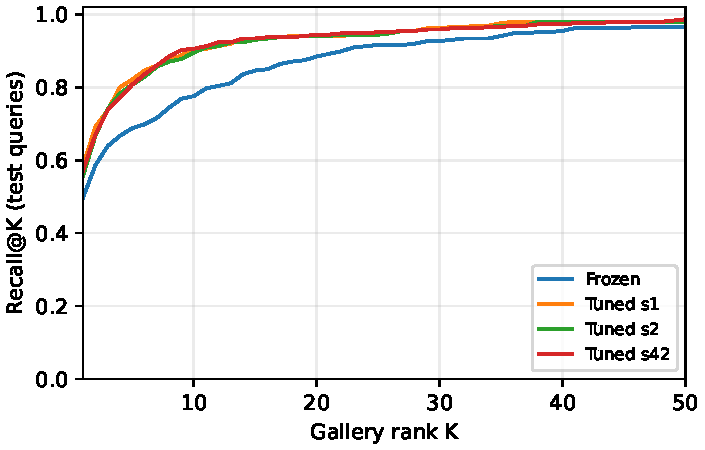
\includegraphics[width=\columnwidth]{fig_fgnet_retrieval_cmc.pdf}
\caption{Fixed-gallery FG-NET test CMC through rank 50 (82 gallery identities, 285 queries).
Curves are generated from cached per-seed ranks, not fitted or selected on test results.
This is not an independent corpus from the verification endpoint. The gallery is not
resampled; query-subject intervals and unresolved training independence are in
Table~\ref{tab:fgnet-retrieval}.}
\label{fig:fgnet-retrieval-cmc}
\end{figure}

\section{Development-Calibrated Verification Errors}\label{sec:supp-errors}
This diagnostic uses the same prespecified person split as retrieval, but constructs
endpoint-age-matched verification positives and negatives separately within each split.
It is a secondary protocol, not the main full FG-NET endpoint: dev retains 279 of 281
eligible positives (39 queried subjects); test retains 282 of 285 (41 subjects), with
one unique impostor per retained positive and identical exact-gap distributions across
classes. Development negative scores alone set thresholds; test scores cannot influence
matching, cutpoints or calibration. Test intervals hold the dev threshold fixed and thus
exclude calibration uncertainty. No deployment-level low-FAR guarantee follows from these
small samples. In particular, 279 dev negatives cannot resolve the nominal 0.1\% point.

% BEGIN GENERATED FGNET ERRORS
\begin{table*}[!t]
\caption{FG-NET test errors at separately dev-calibrated per-model nominal FMR=1\% thresholds, strict score$>$threshold. FA/FR are false accepts/rejects; the observed test FMR need not equal the nominal target. FNMR intervals are both-endpoint subject-bootstrap percentile intervals conditional on the fixed dev threshold; calibration uncertainty is excluded. Blur cutpoints are dev-only, pair sharpness is the lesser endpoint Laplacian variance. Zero-event empirical intervals are not reliable risk bounds. Full exact-year, blur and per-seed results, including the under-resolved nominal 0.1\% point, are in the aggregate artifact; unlabelled pose/scan/collage stay unknown. Training independence is unverified.}
\label{tab:fgnet-errors}
\centering\footnotesize
\begin{tabular}{@{}llccccc@{}}
\toprule
Stratum & Model & FA / negatives & FR / positives & FMR & FNMR & FNMR 95\% CI \\
\midrule
Overall & Frozen & 3/282 & 149/282 & 0.0106 & 0.5284 & $[+0.4327,+0.6272]$ \\
Overall & Tuned s1 & 4/282 & 141/282 & 0.0142 & 0.5000 & $[+0.4135,+0.5931]$ \\
Overall & Tuned s2 & 2/282 & 143/282 & 0.0071 & 0.5071 & $[+0.4235,+0.5971]$ \\
Overall & Tuned s42 & 2/282 & 148/282 & 0.0071 & 0.5248 & $[+0.4364,+0.6206]$ \\
25+ & Frozen & 0/57 & 40/57 & 0.0000 & 0.7018 & $[+0.5322,+0.8704]$ \\
25+ & Tuned s1 & 0/57 & 37/57 & 0.0000 & 0.6491 & $[+0.4385,+0.8537]$ \\
25+ & Tuned s2 & 0/57 & 37/57 & 0.0000 & 0.6491 & $[+0.4478,+0.8367]$ \\
25+ & Tuned s42 & 0/57 & 38/57 & 0.0000 & 0.6667 & $[+0.4615,+0.8710]$ \\
Child-to-adult & Frozen & 0/39 & 33/39 & 0.0000 & 0.8462 & $[+0.7073,+0.9722]$ \\
Child-to-adult & Tuned s1 & 0/39 & 32/39 & 0.0000 & 0.8205 & $[+0.6364,+0.9697]$ \\
Child-to-adult & Tuned s2 & 0/39 & 32/39 & 0.0000 & 0.8205 & $[+0.6315,+0.9714]$ \\
Child-to-adult & Tuned s42 & 0/39 & 32/39 & 0.0000 & 0.8205 & $[+0.6250,+0.9730]$ \\
Blur: low sharpness & Frozen & 0/75 & 41/71 & 0.0000 & 0.5775 & $[+0.4103,+0.7500]$ \\
Blur: low sharpness & Tuned s42 & 0/75 & 42/71 & 0.0000 & 0.5915 & $[+0.4667,+0.7334]$ \\
Blur: middle & Frozen & 1/89 & 46/91 & 0.0112 & 0.5055 & $[+0.3571,+0.6512]$ \\
Blur: middle & Tuned s42 & 0/89 & 45/91 & 0.0000 & 0.4945 & $[+0.3333,+0.6596]$ \\
Blur: high sharpness & Frozen & 2/118 & 62/120 & 0.0169 & 0.5167 & $[+0.3889,+0.6441]$ \\
Blur: high sharpness & Tuned s42 & 2/118 & 61/120 & 0.0169 & 0.5083 & $[+0.3876,+0.6226]$ \\
\bottomrule
\end{tabular}
\end{table*}
% END GENERATED FGNET ERRORS

\section{Historical Scaling and Additional Diagnostics}
\begin{table}[!t]
\caption{Data-scaling law (FaceNet, curated; validation/test fixed; mean $\pm$ std over three seeds).}
\label{tab:supp-scaling}
\centering
\footnotesize
\begin{tabular}{@{}lccc@{}}
\toprule
Train fraction & \# identities & FG-NET large-gap & our.25+ \\
\midrule
frozen & 0 & 0.736 & 0.640 \\
0.10 & $\approx$1{,}500 & 0.846\,$\pm$\,0.002 & 0.816\,$\pm$\,0.003 \\
0.25 & $\approx$3{,}750 & 0.852\,$\pm$\,0.000 & 0.842\,$\pm$\,0.002 \\
0.50 & $\approx$7{,}499 & 0.856\,$\pm$\,0.005 & 0.845\,$\pm$\,0.002 \\
1.00 & $\approx$14{,}998 & 0.848\,$\pm$\,0.001 & 0.835\,$\pm$\,0.003 \\
\bottomrule
\end{tabular}
\end{table}

\begin{table*}[!t]
\caption{Apparent gender/age strata (FaceNet, curated; 95\% paired-bootstrap CI of the gain).}
\label{tab:supp-strata}
\centering
\footnotesize
\begin{tabular}{@{}lccccc@{}}
\toprule
Stratum & $n_{\text{pos}}$ & Frozen & $+$pairs & Gain & 95\% CI \\
\midrule
overall & 5{,}107 & 0.836 & 0.916 & $+$0.080 & [$+$0.075, $+$0.086] \\
apparent F & 3{,}790 & 0.840 & 0.923 & $+$0.084 & [$+$0.077, $+$0.090] \\
apparent M & 1{,}317 & 0.838 & 0.897 & $+$0.059 & [$+$0.048, $+$0.071] \\
age 0--17 & 1{,}123 & 0.750 & 0.880 & \textbf{$+$0.130} & [$+$0.113, $+$0.146] \\
age 18--29 & 3{,}159 & 0.872 & 0.936 & $+$0.064 & [$+$0.058, $+$0.069] \\
age 30--44 & 672 & 0.822 & 0.893 & $+$0.070 & [$+$0.054, $+$0.087] \\
age 45+ & 153 & 0.859 & 0.893 & $+$0.034 & [$+$0.004, $+$0.064] \\
\bottomrule
\end{tabular}
\end{table*}

\begin{table}[!t]
\caption{Hard-negative mining (FaceNet, curated; external benchmarks). $+$hard-neg is mean $\pm$ std over three seeds.}
\label{tab:supp-hardneg}
\centering
\footnotesize
\begin{tabular}{@{}lccc@{}}
\toprule
Metric & Frozen & $+$pairs & $+$pairs$+$hard-neg \\
\midrule
FG-NET large-gap & 0.736 & 0.848 & \textbf{0.868\,$\pm$\,0.004} \\
FG-NET ROC & 0.896 & 0.923 & 0.912\,$\pm$\,0.003 \\
LFW accuracy & 0.969 & 0.950 & 0.925\,$\pm$\,0.005 \\
AgeDB-30 ROC & 0.953 & 0.946 & 0.911\,$\pm$\,0.012 \\
CALFW ROC & 0.948 & 0.949 & 0.898\,$\pm$\,0.015 \\
\bottomrule
\end{tabular}
\end{table}


\section{Partial Matched-Source Control}\label{sec:matched-source}

LOW (1--2-year positive gap) and CROSS ($\geq$25-year positive gap) are mined from
the same VK source. Each arm contains 500 training persons, 1{,}096 unique
positive images, and 600 positive plus 600 negative training pairs. Every
negative keeps its positive A anchor and draws B from age-known images of the
arm's selected people, not only the 1{,}096 selected positive images. This adds
302 negative-only images to LOW and 25 to CROSS: total train images are
1{,}398 versus 1{,}121 (\path{metrics/matched_arm_image_budget_20261002/summary.json}).
The image budget is therefore not fully matched. B age is matched within one year.
The backbone (FaceNet/CASIA), initial weights,
trainable head, learning rate $3\times10^{-5}$, batch size 64, 10 epochs,
preprocessing and held-out FG-NET pairs are shared. We choose the \emph{last}
epoch in both arms; the earlier best-validation comparison selected LOW epoch 1
versus CROSS epoch 10 and is not used for fixed-step inference.

\begin{table}[!t]
\caption{Historical fixed-epoch VK LOW/CROSS control with unequal full image budgets; not the replacement experiment below. Endpoint-age-matched FG-NET
25+ protocol (215 positive/215 negative pairs, 75 subjects). CIs resample
subjects on both sides of a pair; all seeds reuse the same people.}
\label{tab:matched-source}
\centering
\footnotesize
\resizebox{\columnwidth}{!}{%
\begin{tabular}{@{}lcccc@{}}
\toprule
Seed & LOW AUC & CROSS AUC & $\Delta$ AUC & Paired 95\% CI \\
\midrule
1 & 0.8209 & 0.8463 & +0.0254 & [+0.0073,+0.0444] \\
2 & 0.8205 & 0.8455 & +0.0251 & [+0.0079,+0.0429] \\
42 & 0.8203 & 0.8471 & +0.0268 & [+0.0062,+0.0452] \\
Mean $\pm$ SD & 0.8206$\pm$0.0003 & 0.8463$\pm$0.0008 & +0.0257$\pm$0.0009 & --- \\
\bottomrule
\end{tabular}
}
\end{table}

The gain is not a fully causal estimate for longitudinal data: endpoint-age
and quality covariates differ between arms, candidate-person selection may
matter, total training image counts differ, and generic-face plus evaluated
shuffled/co-occurrence controls are absent. Possible mined-train/benchmark identity matches
also require blinded adjudication. The manifest-backed local evidence is
\path{metrics/matched_agegap_fixed10_last/summary.json} and its six run
records; no face crops or biometric templates are part of the submission.

\subsection{Full-image-budget replacement}
Each replacement arm uses 500 recorded people, 1{,}096 total images and 600
positive/600 negative pairs. Within each arm, negative assignment matches
positive ordered endpoint ages and image exposure; between-arm age/quality and
person selection remain different. Original FaceNet/CASIA head fine-tuning uses
uniform row shuffle, batch 64, LR $3\times10^{-5}$, frozen-all BatchNorm statistics,
and epoch 10 (last), on CUDA for all seeds 42/1/2. This changes data construction
and BatchNorm policy relative to the historical experiment, not just hardware.

\begin{table}[!t]
\caption{Replacement CUDA LOW/CROSS control. Means across three checkpoints; paired subject-bootstrap 95\% CI for CROSS minus LOW, not an ensemble AUC. Smaller EER is better.}
\label{tab:oriented-source}
\centering\footnotesize
\resizebox{\columnwidth}{!}{%
\begin{tabular}{@{}llrrrr@{}}
\toprule
Subset & Metric & Frozen & LOW & CROSS & $\Delta$ [95\% CI] \\
\midrule
Overall & AUC & .8870 & .8829 & .8865 & +.0036 [$-.0021,+.0107$] \\
25+ & AUC & .8023 & .7932 & .7963 & +.0031 [$-.0198,+.0261$] \\
25+ & EER & .2791 & .2760 & .2899 & +.0140 [$-.0301,+.0500$] \\
25+ & TAR@FAR .01 & .4465 & .4186 & .3643 & $-.0543$ [$-.1277,+.0868$] \\
25+ & TAR@FAR .001 & .4233 & .3721 & .3581 & $-.0140$ [$-.1209,+.0783$] \\
\bottomrule
\end{tabular}}
\end{table}
Overall has 5{,}308 pairs/82 subjects; 25+ has 430 pairs/75 subjects, all
215 source large-gap positives retained. Both strata share the FG-NET corpus.
All 2{,}000 bootstrap draws are valid, shared across models; positive pairs use
owner multiplicity once, negatives endpoint multiplicity products. Intervals are
conditional on fixed checkpoints/protocol, not a training-seed population, and
are not multiplicity-corrected. ROC thresholds are reselected on evaluation
scores, not development-calibrated deployment thresholds. Interpolated and
discrete-minimax EER coincide at the reported point estimates.
The 25+ AUC leave-one-subject-out CROSS--LOW range is $[-.0011,+.0076]$;
both this sensitivity and the CI fail to establish superiority. CROSS versus
frozen AUC difference is $-.0060$ with CI $[-.0324,+.0217]$.
No causal source claim or training-identity independence is established.
Evidence: \path{metrics/oriented_cuda_fgnet_20261004/summary.json} and native
manifest; full score/embedding artifacts are private biometric data, not public
submission attachments. Generic/co-occurrence controls and human overlap
adjudication remain open.

\subsection{Fixed-permutation supervision-noise sensitivity}
Using the same full-budget CROSS images, negative pairs, held-out data and
fixed10/last/frozen-BatchNorm protocol, permutation seed 42 changes 576 of 600
positive-label pairs to different recorded persons, retaining 24 genuine pairs.
This is 96\% artificial positive-label noise (48\% of all rows), not an estimate
of mining error. Training seeds 42/1/2 are distinct from the permutation seed.
On the shared endpoint-age-matched FG-NET protocol, mean AUC falls from 0.8865
to 0.8653 overall (noise--clean $-0.0212$, paired subject 95\% CI
$[-0.0260,-0.0164]$), and from 0.7963 to 0.7748 on 25+
($-0.0216$, CI $[-0.0319,-0.0114]$). All three per-checkpoint 25+ AUC
intervals exclude zero; leave-one-subject-out mean differences remain negative
($[-0.0230,-0.0199]$). However, 25+ EER changes from 0.2899 to 0.3070
($+0.0171$, CI $[-0.0039,+0.0409]$), TAR@FAR1\% from 0.3643 to 0.3411
($-0.0233$, CI $[-0.0962,+0.0061]$), and TAR@FAR0.1\% from 0.3581 to 0.3333
($-0.0248$, CI $[-0.0857,+0.0067]$): those intervals include zero.
All 2{,}000 shared subject-bootstrap draws are valid in both strata;
conditioning, endpoint weights and test-derived threshold limitations are
as above. The result supports sensitivity to this specific artificial permutation,
not robustness across permutations, empirical annotation precision, co-occurrence
control or causal source superiority. Evidence:
\path{metrics/oriented_noise_cuda_fgnet_20261004/summary.json} and native manifest;
private score/embedding artifacts are not public attachments.

\section{Figures Referenced from the Main Paper}\label{sec:figs}
These five plots visualize the headroom, data-scaling, objective, apparent-attribute and external-benchmark results. Secondary scaling/fairness/hard-negative tables are kept here so the main manuscript remains focused and within the 10-page limit.

\begin{figure}[!t]
\centering
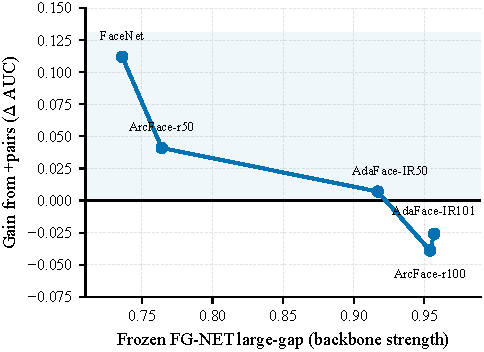
\includegraphics[width=\columnwidth]{fig_headroom.pdf}
\caption{Exploratory one-seed headroom curve: the $+$pairs gain on FG-NET large-gap declines overall but not monotonically as the frozen backbone strengthens. This plot motivates the planned fixed-budget mechanism matrix; it does not by itself establish saturation or distinguish ceiling, plasticity and forgetting.}
\label{fig:headroom}
\end{figure}

\begin{figure}[!t]
\centering
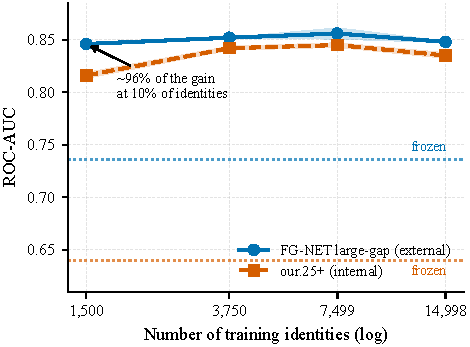
\includegraphics[width=\columnwidth]{fig_scaling_layout_v2.pdf}
\caption{Exploratory scaling sweep: external (FG-NET large-gap) and internal (our.25+) ROC-AUC vs.\ training identities (log scale). The recorded 10\% point reaches roughly 96\% of the gain, but intermediate checkpoints were overwritten; shaded bands show the recorded seed variation, not yet a fully checkpoint-verifiable result.}
\label{fig:scaling}
\end{figure}

\begin{figure}[!t]
\centering
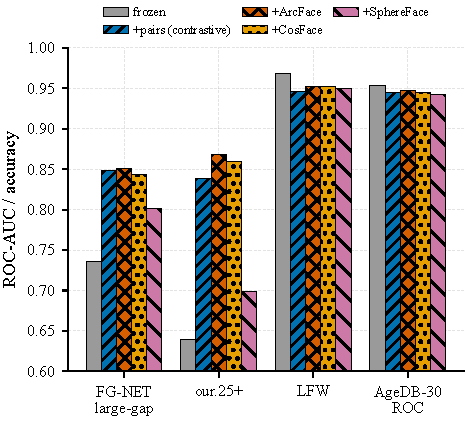
\includegraphics[width=\columnwidth]{fig_sota.pdf}
\caption{Objective comparison: contrastive, ArcFace and CosFace have similar point estimates on historical cross-age transfer; SphereFace (hardest to optimize, no $\lambda$-annealing) trails. ArcFace/CosFace forget slightly less on easy benchmarks.}
\label{fig:sota}
\end{figure}

\begin{figure}[!t]
\centering
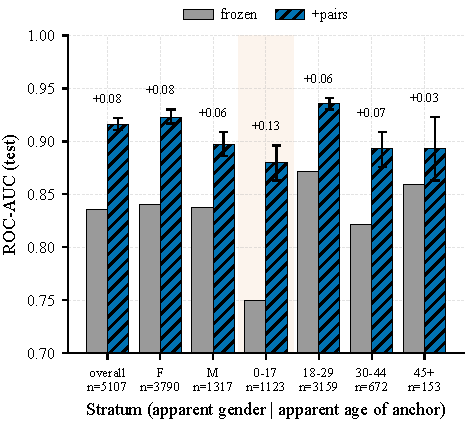
\includegraphics[width=\columnwidth]{fig_fairness.pdf}
\caption{Apparent-demographic audit: frozen vs.\ $+$pairs ROC-AUC across apparent gender/age strata. Every stratum improves; the largest gain is for the youngest (0--17) group, where the frozen baseline is weakest. Error bars are the 95\% paired-bootstrap CI of the gain and $n$ is positive pairs per stratum (the sparse 45+ stratum, $n{=}153$, has a correspondingly wide interval).}
\label{fig:fairness}
\end{figure}

\begin{figure}[!t]
\centering
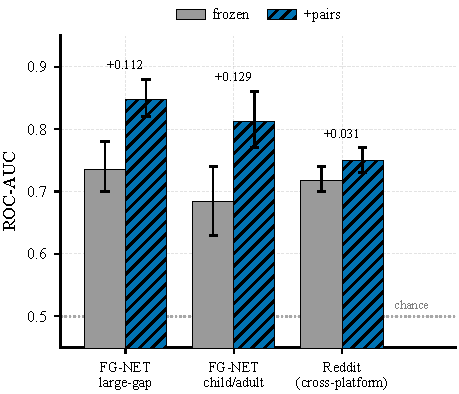
\includegraphics[width=\columnwidth]{fig_external_layout_v2.pdf}
\caption{Historical random-impostor external results, not the corrected endpoint-age-matched FG-NET headline. The $+$pairs gain over the frozen baseline (with the historical 95\% CIs) is shown for FG-NET large-gap, a child$\leftrightarrow$adult subset of the same FG-NET corpus, and a separate cross-platform Reddit source. The two FG-NET estimates are dependent; these gains must not be substituted for corrected-protocol results.}
\label{fig:external}
\end{figure}

\bibliographystyle{IEEEtran}
\bibliography{../../../shared/refs}

\end{document}
